\chapter{\library{Mirage}: Echo-aware Sound Source Localization}\label{ch:mirage}

\openepigraph{Scanning all around [...]\\
Ancient blocks of sound\\
Mirage}{Meat Puppets, \textit{Mirage}}

\vspace{-2.5em}
\newthought{Synopsis} \marginpar{%
    \footnotesize
    \textbf{Keywords:} Sound Source Localization, Image Microphones, Acoustic Echoes, TDOA Estimation.
    \\\textbf{Resources:}
    \begin{itemize}
        \item \href{https://ieeexplore.ieee.org/document/8683534}{Paper}
        \item \href{https://github.com/Chutlhu/mirage}{Code}
        \item \href{https://sigport.org/documents/mirage-2d-sound-source-localization-using-microphone-pair-augmentation-echoes}{Poster}
        \item \href{https://www.youtube.com/watch?v=SfEmwqxxpYg}{HARU Robot presentation}
    \end{itemize}
} \synopsisChMirage

\mynewline
Together with~\cref{ch:lantern}, this chapter describes methods and results published in~\cite{di2019mirage}, which considers only stereophonic recordings.
In this sense, this chapter provides an application for \acs{LANTERN}, the learning-based echo estimation method presented in the above mentioned chapter.

% \\Later, the proposed approach was  extended to multi-microphone recordings in a collaboration with Randy Gomez from the Honda Research Institute.
% In particular, the method was tested considering the microphone array of the autonomous robot platform called \textit{HARU}\citeonly{ackerman2018haru, gomez2018haru}, \marginpar{
%     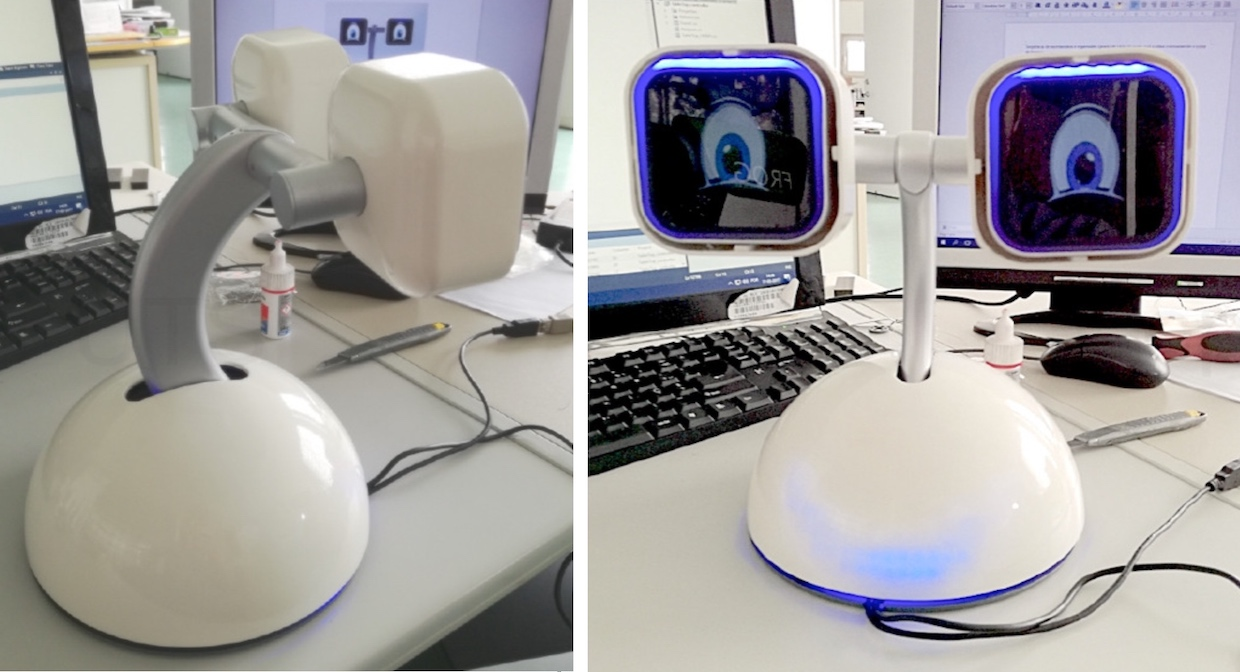
\includegraphics[width=\linewidth]{mirage/haru.jpeg}
%     \captionof{figure}{The HARU Robot.}
%     \label{fig:mirage:haru}
% } (See~\cref{fig:mirage:haru})
% The robot is fitted with cameras and a microphone array for visual and audio sensing.
% The array is circular with 6.5~cm radius, featuring 7 sensors.
% The partner agreed on using its technology to see the impact of echo-aware sound source localization.
% Unfortunately, we found some issues in annotating and using the recorded data.
% Therefore our investigation here is limited to synthetic data.

% The results of this study were described in an internal technical report~\citeonly{di2019honda}.


\section{Literature review in echo-aware Sound Source Localization}
Common to most sound source localization approaches reviewed in ~\cref{sec:application:localization} is the challenge posed by reverberation.
It is typical to observe that \acf{DOA} estimation degrades with increasing acoustic reflections~\citeonly{chen2006time}.
For these reasons, most sound source localization methods regard reverberation, and in particular acoustic echoes, as a nuisance.
Some prior works, \eg/, \citeonly{rui2004time, chen2006time, zhang2007maximum}, modeled the reverberation as a noise term.
However, the commonly used dereverberation methods do not reduce strong early echoes.
Alternatively, approaches in~\citeonly{weinstein1994iterative, taghizadeh2015spatial, salvati2016sound} attempt to solve \SSL/ by estimating the full \RIRs/, which is known to be a very difficult task.

\mynewline
Instead, echo-aware sound source localization methods take another direction:
they exploit the closed-form relation between echo timings and the audio scene geometry as expressed in the \acf{ISM}.
Early works such as~\citeonly{korhonen2008acoustic, ribeiro2010turning, ribeiro2010using, svaizer2011use} use knowledge form the room geometry to estimate the position of the sound source with respect to the array.
This idea was subsequently extended in later works, reducing the amount of prior knowledge required or addressing different applications.
The authors of \citeonly{nakashima2010localization} study the \SSL/ problem in binaural recordings.
To improve localization, they propose to used ad-hoc reflectors as artificial \textit{pinnae} and a simple reflection model.
In the work~\citeonly{krekovic2016echoslam}, the authors address the problem of Acoustic \ac{SLAM}\sidenote{
    Acoustic \ac{SLAM} enables the estimation of a moving robot’s position in relation to a number of external acoustic sources~\citeonly{evers2018acoustic}.
} using echoes.
The authors of~\citeonly{an2018reflection} leverage on cameras, depth sensors, and laser sensors to identify reflectors and build a corresponding acoustic model that is used later for localizing sources.
Finally, in a very recent work, the well-known \ac{MUSIC} framework is modified to account for an echo model in the spherical harmonic representation~\citeonly{birnie2020reflection}

\mynewline
All the above mentioned echo-aware methods are explicitly knowledge-driven, namely, they use closed-form solutions based on physics, acoustics, and signal processing models.
The benefit of manipulating ``simple'' models is however paid by strong assumptions, simplifications and a need for hand-crafted features.
In order to overcome these limitations, data-driven methods have been proposed to address \SSL/ (see~\cref{sec:application:localization}).
This approach leverages  training datasets to implicitly learn the mapping from audio features to the source position.
Such data can be obtained from real recordings or using physics-based simulators.
These methods were showed to overcome some limitations of physics-based model, especially when some assumptions are violated.
However, they are typically trained for specific applications and use-cases (\eg/, specific array geometries, acoustic conditions, \etc/) and fail whenever test conditions strongly mismatch training conditions.

\section{Proposed approach}
In this work, we propose to combine the best of the two worlds:
\begin{itemize}
    \item to use a data-driven model to estimate sound propagation parameters;
    \item to use a knowledge-driven model to map such parameters to the source's \ac{DOA}.
\end{itemize}
Let us first introduced a simple yet common scenario:
\marginpar{%
    \centering
    \footnotesize
    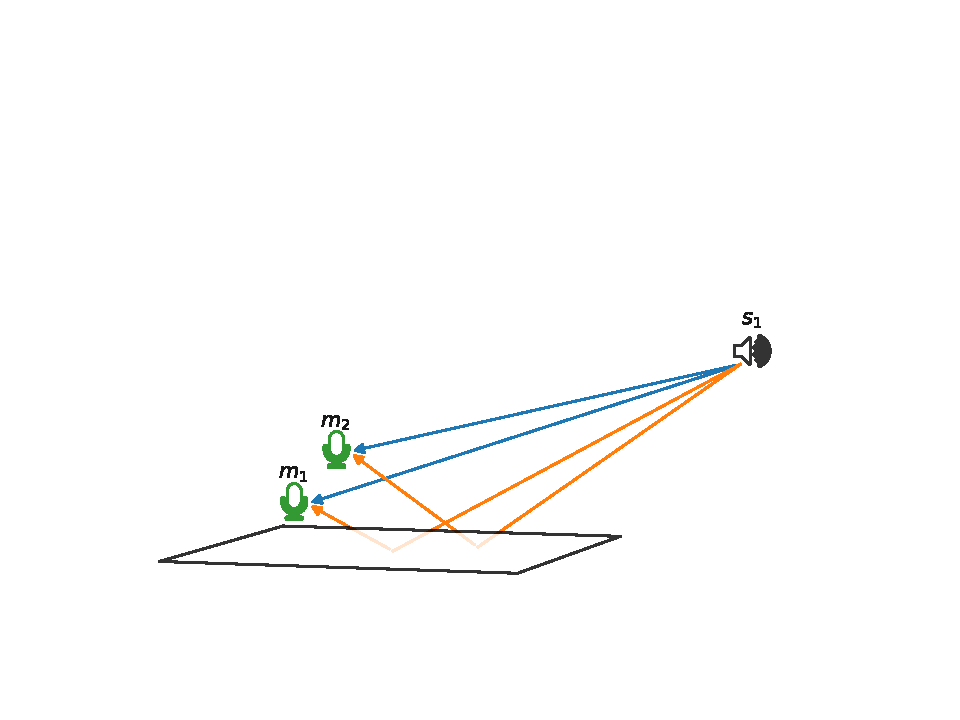
\includegraphics[trim={50 70 50 150},clip,width=\linewidth]{mirage/scene.pdf}
    \captionof{figure}{%
        Typical setup with one sound source recorded by two microphones.
        The illustration shows the direct sound path (blue lines) and the resulting first-order echoes (orange lines).}
    \label{fig:mirage:scene}
}
two microphones, one source, and a nearby reflective surface, as illustrated in~\cref{fig:mirage:scene}.
This may occur when the sensors are placed on a table or next to a wall.
Striking examples of this scenario are smart table-top devices, such as Amazon Echo, Google Home, \etc/.
The reflective surface is assumed to be the most reflective and closest one to the microphones in the environment, generating the strongest and earliest echo in each microphone.
Under this stereophonic \textit{close-surface} model, we ask the following questions.

\questionpar{Can early echoes be estimated from two-microphone recordings of an unknown source?}
To answer this question, we propose to use the class of deep learning models \acs{LANTERN}, presented in~\cref{ch:lantern}.
These models are trained on a close-surface dataset to estimate the first early echoes per channel from audio features.

\questionpar{Can early echoes be used to estimate both the azimuth and elevation angles of the source?}
To answer the second question, we propose the \acf{MIRAGE} framework.
It exploits echo times of arrival by expressing them as \acp{TDOA} in a \textit{virtual 4-microphone array} formed by the true microphone pair and its image with respect to the reflective surface.
This model is based on the \textit{image microphones} model (See~\cref{sec:separake:sota}).
Note that answering this question is can \textit{impossible} task in free- and far-field stereophonic conditions , due to the well known spatial ambiguity of a single \ac{TDOA}, referred to as the \textit{cone of confusion}~\citeonly{Bregman:1994tz}

\section{Background in microphone array SSL}\label{sec:background}
In this section, we briefly review some necessary background in microphone array \ac{SSL}.
Let us assume a microphone array of $\numMics$ sensors is placed inside a room and records the sound emitted by one static point sound source ($\numSrcs=1$).
Recalling the signal model presented in~\cref{eq:estimation:signalmodel}, the relationship between the signal $\mic_\idxMic$ recorded by the $\idxMic$-th sensor placed at fixed position $\positionMicrophone_\idxMic$ and the signal $\src$ emitted by the source at fixed position $\positionSource$ writes
\begin{equation}\label{eq:mirage:signalmodel}
    \begin{aligned}
        \tildex_i(t) &= (\tildeh_i \convCont \tildes)(t) + \tilden_i(t)\\
        \tildeh_i(t) &= \echoModelTimeSimple{i} + \tilde{\varepsilon}_i(t),
    \end{aligned}
\end{equation}
where $\nse_\idxMic$ denotes possible measurement noise and $\varepsilon_i[k]$ collects later echoes, the reverberation tail, diffusion, and undermodeling noise.
In this work, we will consider only the first strongest echo, therefore $R = 1$.
Note that for $r=0$ denotes the direct propagation path, where $\tau_i^(0)$ is the direct path's time of arrival from the source to the $\idxMic$-th microphone, and $\alpha^{(0)}_{\idxMic}$ captures both the sound wave attenuation and air absorption effects.
In the remainder of this chapter, we make the approximation of $\alpha_i^{(\idxEch)}$ being frequency-independent.

\subsection{2-channel 1D-SSL}\label{subsec:mirage:1D-SSL}
\newcommand{\tdoa}{\ensuremath{\tau_\mathtt{TDOA}}}
\newcommand{\aoa}{\ensuremath{\vartheta}}
Let us first consider the case of stereophonic recordings ($\numMics=2$).
Under far-field assumption, traditional \SSL/ methods use the \acf{TDOA},
\begin{equation*}
    \tdoa \eqdef \tau^{(0)}_2 - \tau^{(0)}_1\quad\text{[second]}
    ,
\end{equation*}
as a proxy for the estimation of the \ac{AOA}, $\aoa$, since:
\begin{equation}\label{eq:mirage:aoa}
    \vartheta \approx \arccos \kparen{\speedOfSound \: \tdoa \: / \: \distMicMic }\quad\text{[rad]},
\end{equation}
where $\speedOfSound$ is the speed of sound and $\distMicMic$ is the inter-microphone distance, considered small compared to the source's distance.
\begin{figure}
    \begin{sidecaption}[]{
        Illustration of the relation between \ac{DOA} and \ac{TDOA} with ones source and two microphones.
        Knowing the distance $\distMicMic$ between the two microphones, simple trigonometry yields the \ac{AOA} $\vartheta$ according to~\cref{eq:mirage:aoa}.
    }[fig:mirage:gcc]
        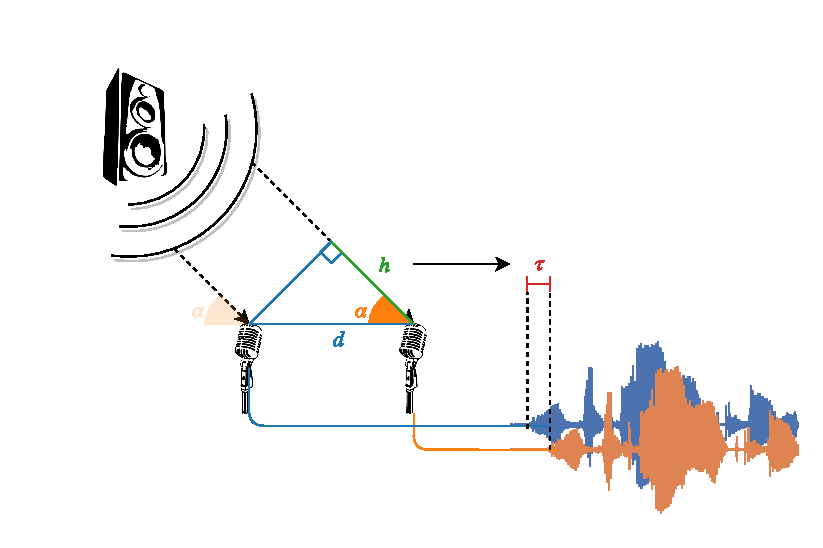
\includegraphics[width=\linewidth]{mirage/tdoa_microphone.pdf}
    \end{sidecaption}
\end{figure}
\\Then, \SSL/ reduces to estimating the \ac{TDOA}, which can be done by a \ac{CC}-based methods, \eg/, the \acf{GCC-PHAT} method\marginpar{
    \footnotesize\itshape
    The ``generalized'' cross-correlation methods add weighting functions (\eg/ the \acf{PHAT}, or the smoothed coherence transform (SCOT)) to the frequency-domain \ac{CC}.
    Their purpose is to improve the estimation of the time delay depending on specific characteristics of the signal and noise.
    See~\citeonly{chen2006time} for an overview.
} \citeonly{knapp1976generalized, blandin2012multi}.
Given the \STFT/ $\MIC_1$ and $\MIC_2$ of the two microphones signals, the \ac{CC} and \ac{GCC-PHAT} \textit{angular spectra} are defined as:
\begin{equation}\label{eq:mirage:cc}
    \Psi_\mathtt{CC}(\tau) = \sum_{k,l} \MIC_1[k,l] \MIC_2^{*}[k,l] \cste^{-\csti 2  \pi f_k \tau}
    ,
    \end{equation}
\begin{equation}\label{eq:mirage:gccphat}
    \Psi_\mathtt{PHAT}(\tau) = \sum_{k,l}\frac{\MIC_1[k,l] \MIC_2^{*}[k,l]}{\kvbar{ \MIC_1[k,l] \MIC_2^{*}[k,l] }} \cste^{-\csti 2  \pi f_k \tau}
    ,
\end{equation}
where $*$ denotes the complex conjugate, $[k,l]$ indexes a \ac{TF} bin of the \STFT/ and $f_k$ is the $k$-th natural frequency in the \STFT/.
\\The weighting function $1 / \kvbar{ \MIC_1[k,l] \MIC_2^{*}[k,l]}$ is called \acf{PHAT}.
This function was introduce to suppress the source's autocorrelation component from the angular spectrum.
\\Then, the \ac{TDOA} estimate is given by
\begin{equation*}
    \hat{\tau}_\mathtt{TDOA} = \arg \underset{\tau}{\max} \; \Psi(\tau)
    ,
\end{equation*}
with $\Psi$ being either $\Psi_\mathtt{CC}(\tau)$ or $\Psi_\mathtt{PHAT}(\tau)$.
Note that these functions can also be expressed directly as a function of the \ac{AOA} using \eqref{eq:mirage:aoa}, hence the term \textit{angular spectrum}.
Despite the theoretical limitation of \ac{CC}-based methods presented in~\citeonly{chen2006time}, they are known to work well in practice.
Moreover, it was showed to be state-of-the-art for \ac{SSL} in a large benchmark study~\citeonly{blandin2012multi}.

\subsection{Multichannel 2D-SSL}\label{subsec:mirage:2D-SSL}
When more microphones are available and the microphone array is compact and not linear\sidenote{
    In the case where the microphones are complanar, the angle can be estimated up to an ``up-down'' ambigity.
}, 2D-\ac{SSL} can be envisioned.
A possible approach is to use 1D-\ac{SSL} on all pairs and combine their results, a principle which was successfully applied in the \acf{SRP-PHAT} method \citeonly{dibiase2001robust}.

\begin{figure}
    \begin{sidecaption}[t]{
        Illustration of the different \acp{DOA} at each microphone pairs attending one sound source.
        Knowing the position of the microphones, the angle with respect to a reference frame can be deduced in closed-form.
    }[fig:mirage:srp]
    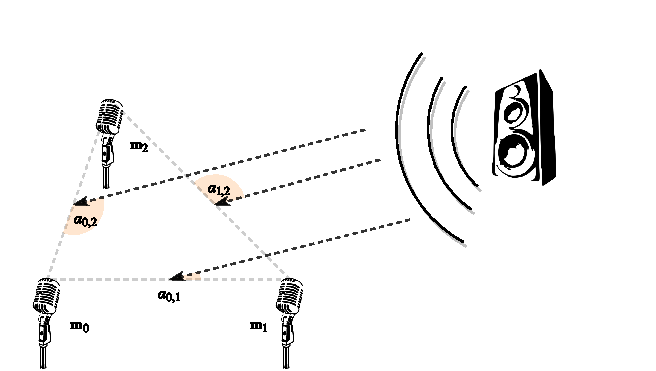
\includegraphics[width=\linewidth]{mirage/srp-phat_aggregation.pdf}
\end{sidecaption}
\end{figure}

\mynewline
The \ac{SRP-PHAT} method returns the source's \ac{DOA}, namely azimuth-elevation pair $(\theta, \phi)$, by estimating \acp{TDOA} in all microphone pairs.
In order to achieve this, it requires the geometry of the microphone array to be known.
In a nutshell, this algorithm aims to estimate a \textit{global angular spectrum} $\Psi_{\mathtt{SRP}}(\theta,\phi)$ in the polar coordinates system with respect to a reference frame in the array, typically centered at its barycenter.
This function will exhibit a local maximum in the direction of the active source.
\\The algorithm can be decomposed into in the following steps:\marginpar{
    \footnotesize\itshape
    See \href{http://bass-db.gforge.inria.fr/bss_locate/}{\library{MBSSLocate}\ExternalLink} for a free MATLAB implementation and comprehensive documentation of this algorithm.
}
\begin{enumerate}
    \item a global grid of \acp{DOA} candidates is defined according to a desired resolution and computational load;
    \item for each pair of microphones, a local set of \acp{AOA} (hence, \acp{TDOA}) is defined based on the above chosen \acp{DOA} and the input geometry;
    \item a TDOA-based algorithm (\eg/ \ac{GCC-PHAT}) is used to compute the associated local angular spectrum;
    \item all the local contributions (a collection of local $\Psi_\mathtt{GCC}(\tau)$) are geometrical aggregated and interpolated back to the global \ac{DOA} grid to form $\Psi_{\mathtt{SRP}}(\theta,\phi)$;
    \item the \acs{DOA}(s) maximizing $\Psi_\mathtt{SRP}$ is (are) used as estimate(s).
\end{enumerate}
% This algorithm can be seen under the \textit{divide-and-conquer paradigm}:
% ``at the leaves'', the \ac{GCC-PHAT} method provides \ac{TDOA} for each microphone pair;
% the ``merge'' operation consists in aggregating \ac{TDOA} defined on a different axis based on the knowledge of the array geometry.
% Finally, we stress that this algorithm is independent of the method used to estimate the \ac{TDOA}.

\section{Microphone Array Augmentation with Echoes}\label{sec:mirage:mirage}
We now introduce the proposed concept of \MIRAGEdef/.
In the well-known \acf{ISM} all the reflections are treated as mirror images of the true source with respect to reflective surfaces, emitting the same signal.
\marginpar{%
\centering
\footnotesize
    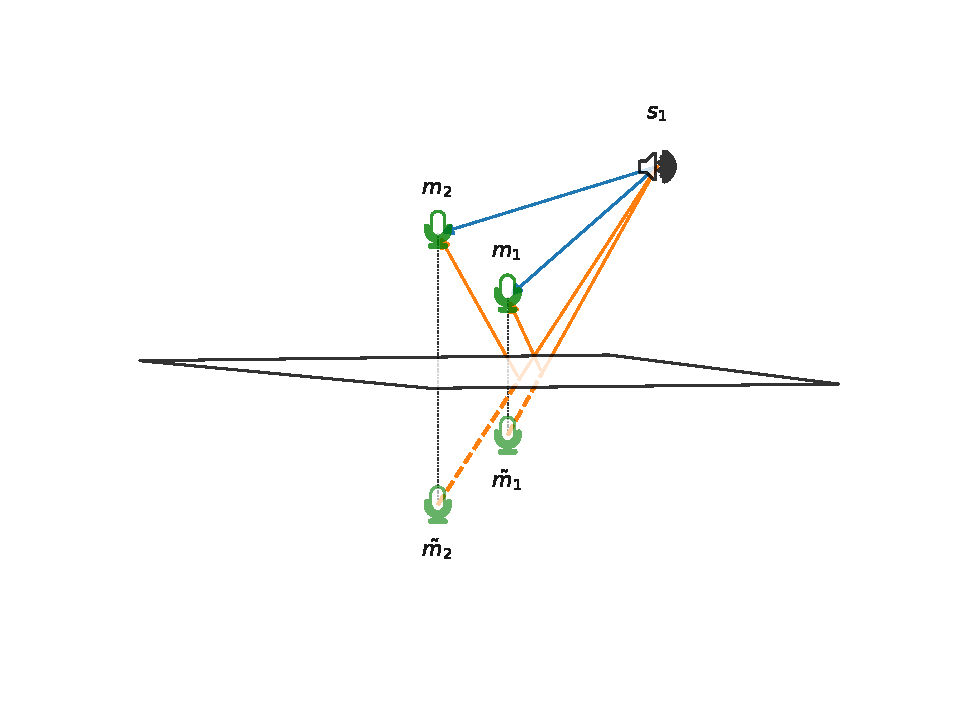
\includegraphics[trim={90 75 40 50},clip,width=\linewidth]{mirage/mirage.pdf}
    \captionof{figure}{%
        Illustration of the images $\mathring{\positionMicrophone}_1$ and $\mathring{\positionMicrophone}_2$ of microphones $\positionMicrophone_1$ and $\positionMicrophone_2$ in the presence of a reflective surface and a source.
        Blue lines correspond to direct paths, orange lines correspond to echo paths.}
    \label{fig:mirage:mirage}
}
We will employ here a less common but equivalent interpretation to \ISM/, namely, the image-microphone model (see~\cref{sec:separake:sota})
As illustrated in~\cref{fig:mirage:mirage}, image microphones are mirror images of the true microphones with respect to reflective surfaces.
In this view, the echoic signal received at a true microphone is the sum of the anechoic signals received at this microphone and its images.
If we consider the virtual array consisting of both true and image microphones, multiple microphone pairs are now available.
For each of them, it is then possible to define a corresponding time difference of arrival.
Among them, we will refer to the one defined in~\cref{sec:lantern:simple}, that is,
Therefore, we have:
\begin{equation}
    \begin{aligned}
        \tau_\mathtt{TDOA}  &= \tfrac{1}{c} \norm{\positionMicrophone_2 - \positionSource} - \tfrac{1}{c} \norm{\positionMicrophone_1 - \positionSource} = \tau_2^{(0)} - \tau_1^{(0)},\\
        \tau_\mathtt{iTDOA} &= \tfrac{1}{c} \norm{\mathring{\positionMicrophone}_2 - \positionSource} - \tfrac{1}{c} \norm{\mathring{\positionMicrophone}_1 - \positionSource} = \tau_2^{(1)} - \tau_1^{(1)},\\
        \tau_{\mathtt{TDOE}_1}  &= \tfrac{1}{c} \norm{\mathring{\positionMicrophone}_1 - \positionSource} - \tfrac{1}{c} \norm{\positionMicrophone_1 - \positionSource} = \tau_1^{(1)} - \tau_1^{(0)}\\
        \tau_{\mathtt{TDOE}_2}  &= \tfrac{1}{c} \norm{\mathring{\positionMicrophone}_2 - \positionSource} - \tfrac{1}{c} \norm{\positionMicrophone_2 - \positionSource} = \tau_2^{(1)} - \tau_2^{(0)}
    \end{aligned}
\end{equation}
where $\mathring{\positionMicrophone}_i$ denotes the position of the image of $\positionMicrophone_i$ with respect to the reflector.
It is easy to see that $\tau_{\mathtt{TDOE}_2} =  \tau_{\mathtt{TDOE}_1} + \tau_\mathtt{iTDOA} - \tau_\mathtt{TDOA}$.
Therefore, we will consider only the set $V = \klist{\tau_{\mathtt{TDOA}}, \tau_{\mathtt{iTDOA}}, \tau_{\mathtt{TDOE}_1}}\in\mathbb{R}^3$.
These three quantities are directly connected to \RIRs/, as illustrated in~\cref{fig:mirage:rirs_tdoa}.\marginpar{%
\centering
\footnotesize
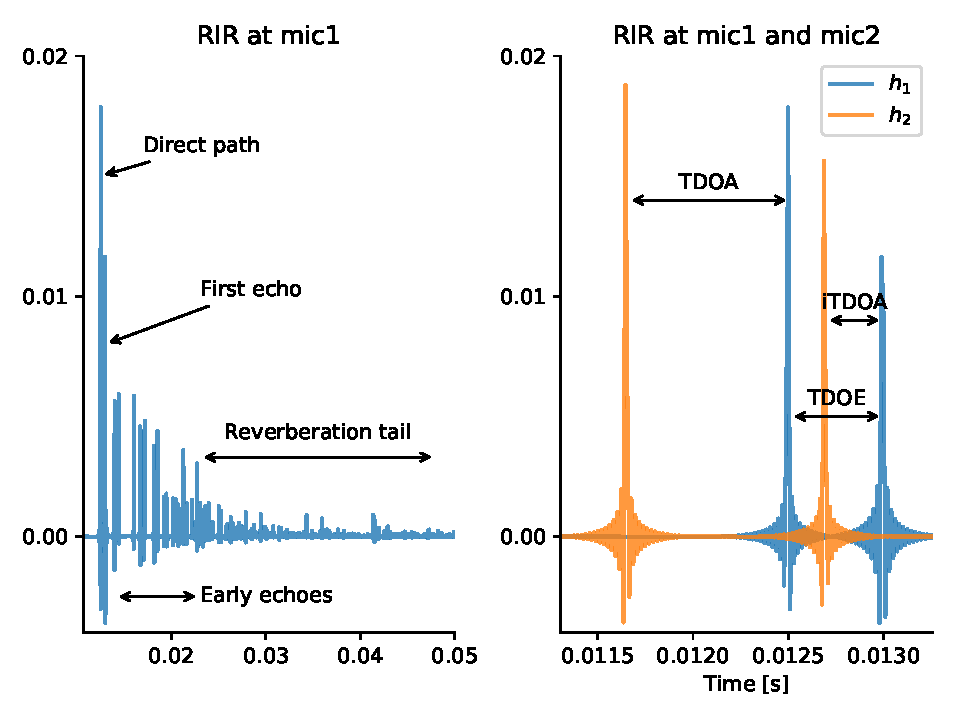
\includegraphics[trim={82mm 0 0 0},clip,width=\linewidth,height=7cm]{mirage/rirs.pdf}
\captionof{figure}{%
    Superposition of two \acp{RIR} and visualization of time difference of arrival between direct paths (\ac{TDOA}), first echoes (\ac{iTDOA}) and direct path and first echo (\ac{TDOE}).}
\label{fig:mirage:rirs_tdoa}
}%
% Note that they are the same estimated by the \acs{LANTERN} \ac{DNN} presented in~.

\mynewline
To learn the parameters $V$, we consider the \acs{LANTERN} data-driven approaches presented in~\cref{ch:lantern}.
It consists in a class of \ac{DNN} architectures trained to perform multi-target regression from the input audio features \acf{ILD} and \acf{IPD} to to the parameters $V\in\bbR^3$.
In fact, those models were proposed exactly to address the task of estimating the first and strongest echo per channel in a close-surface scenario.

\mynewline
Following the 2D-\SSL/ scheme described in \cref{subsec:mirage:2D-SSL} and given the virtual microphone-array geometry (which depends on the relative position of microphones to the surface), $V$ can in principle be used to estimate the 2D direction of arrival of the source.
To this end, the 3 real-valued estimates in $V$ are converted into \textit{virtual} local angular spectra (see~\cref{subsec:mirage:2D-SSL}).
In the first investigation of~\citeonly{di2019mirage}, we proposed to use Gaussians functions centred at the estimates $\hat{V}$ with variances equal to the prediction errors made by the \ac{DNN} on the validation set.
Later, we modified the networks in order to estimated both these means and the variances, as explained in~\cref{sec:lantern:robust}.

% In the~\cref{ch:lantern}, we introduced a learning-based method to estimate $V$ using audio features obtained from only two microphones.
% Given a microphone pair, the local maximum of angular spectrum $\Psi_\text{PHAT}$ corresponds to the \ac{TDOA}.
% Moreover, peaks corresponding to the early reflection are also present.
% \cref{fig:mirage:noise_ang_spec} shows the $\Psi_\mathtt{CC}$'s and the $\Psi_\mathtt{PHAT}$'s angular spectra for synthetic data where the source signal is noise or speech for all the pairs of the HARU's circular microphone array.
% The location of the quantities in $V$ are highlighted with vertical dotted lines.
% Theoretically, when only the first reflection are considered ($K=1$), the position of the peaks in the angular spectra correspond to
% $\tau_\mathtt{TDOA}$, $\tau_\mathtt{iTDOA}$, $\tau_\mathtt{TDOA} - \tau_{\mathtt{TDOE}, 1}$, and $\tau_\mathtt{TDOA} + \tau_{\mathtt{TDOE}, 2}$.
% It is important to note that for speech signals, $\Psi_\text{PHAT}$ removes the auto-correlation part in order to promote a sharp peak at the position of the \ac{TDOA}.
% Since acoustic echoes increase the auto-correlations of the signal in one microphones, the \acs{PHAT} transform tends to lower their contribution, so that their peaks are not distinguishable from spurious ones.
% \begin{figure}
%     \begin{fullwidth}
%         \centering
%         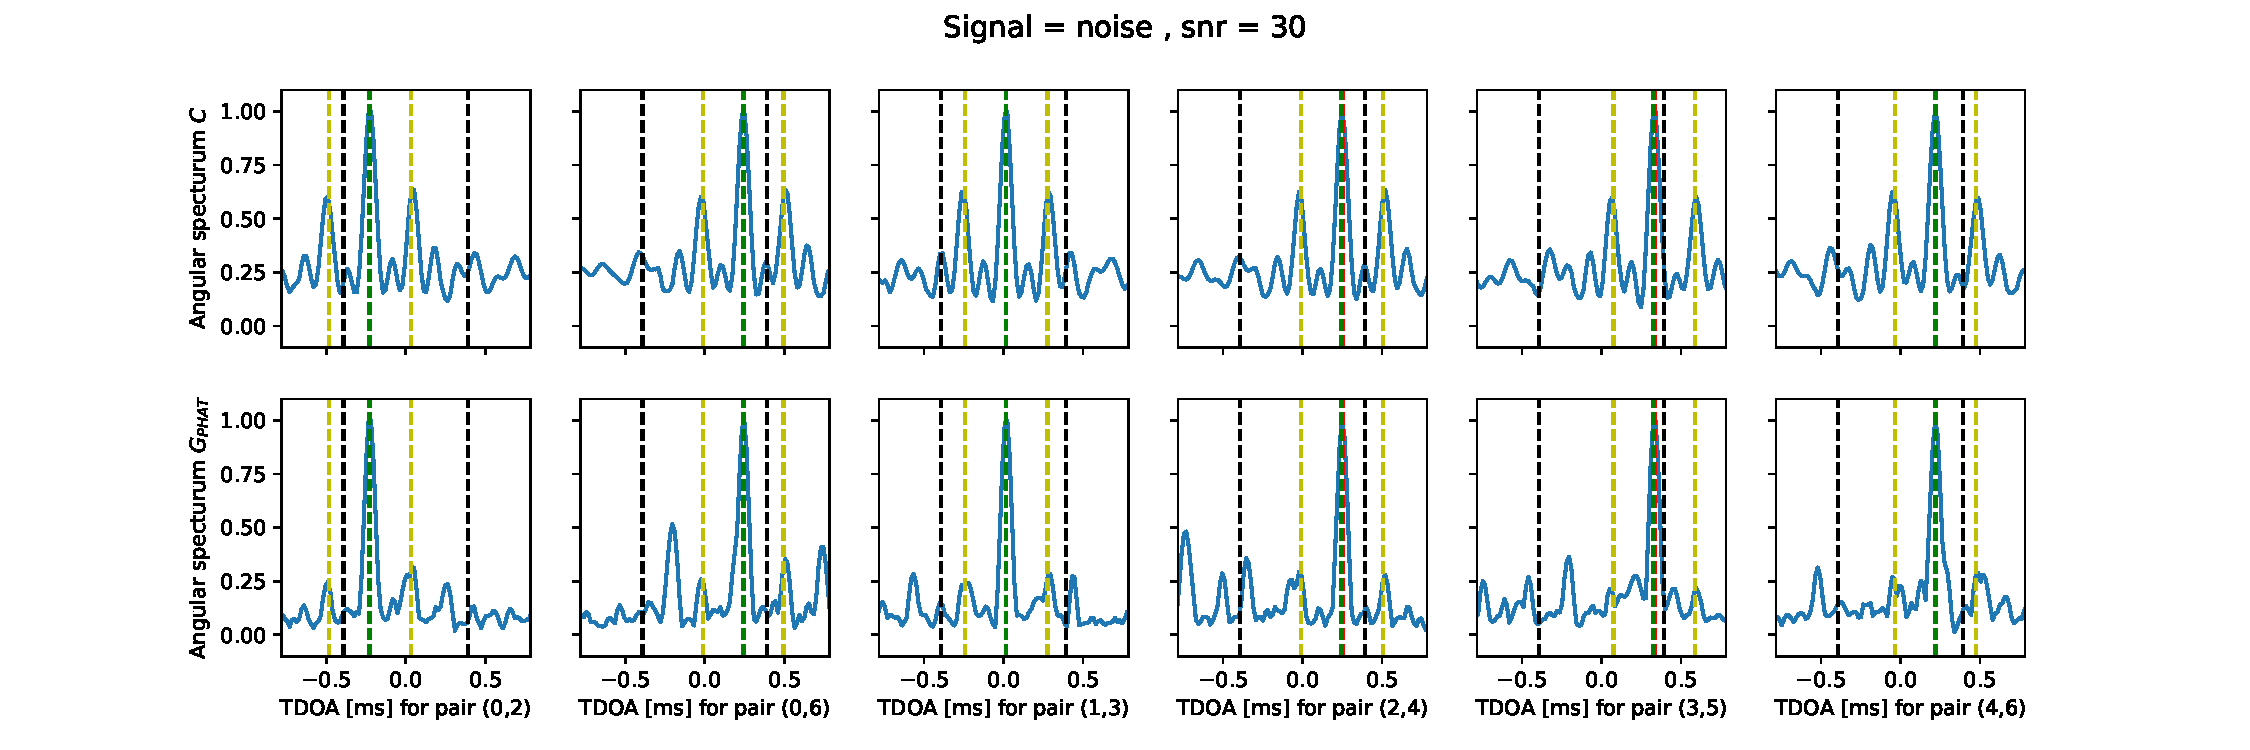
\includegraphics[trim={0mm 0 0mm 0},clip,width=\linewidth]{mirage/echo_hunting_broadband.pdf}
%         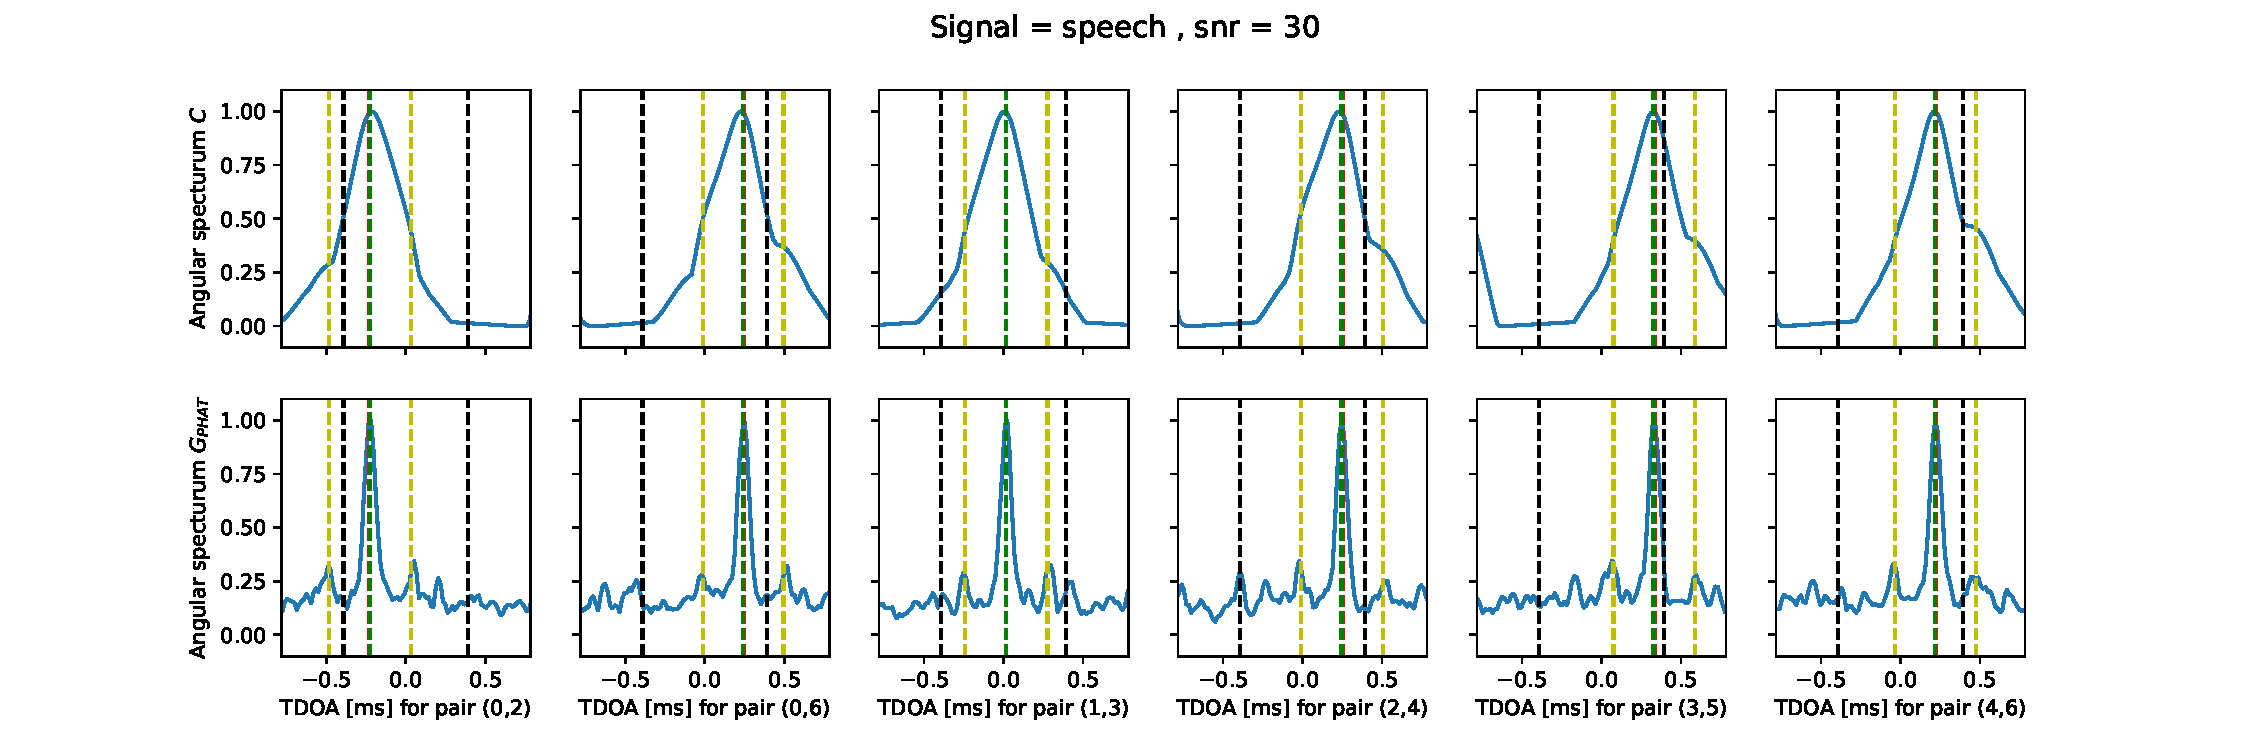
\includegraphics[trim={0mm 0 0mm 0},clip,width=\linewidth]{mirage/echo_hunting_speech.pdf}
%         \caption{
%             Angular Spectra $\Psi_\mathtt{CC}$ and $\Psi_\texttt{PHAT}$ for different pairs of microphone in the HARU array using synthetic \RIRs/ and \textit{white noise} (top) and \textit{speech} (botton) signal .
%             Vertical lines mark the positions of  $\tau_\mathtt{TDOA}$ (red), $\tau_\mathtt{iTDOA}$ (green), $\tau_\mathtt{TDOA}-\tau_\mathtt{TDOE,1}$ (yellow) and $\tau_\mathtt{TDOA}+\tau_\mathtt{TDOE,2}$ (yellow) are marked with vertical lines.
%             The black vertical lines correspond to the maximum TDOA given the pair distance, \textit{i.e.} corresponding to the AOA $ = \{0, 2\pi\}$}
%         \label{fig:mirage:noise_ang_spec}
%     \end{fullwidth}
% \end{figure}


\subsection{Experimental Results}\label{sec:mirage:exp}
In this section we will report the experimental results for the proposed approach.
At first, we will consider the continuation of the investigation started in~\cref{sec:lantern:simple}, namely, the analysis is limited to stereophonic recordings in a single-source close-surface scenario.

Here we compare the \ac{MIRAGE} approach using the \acs{LANTERN} \ac{MLP} (MIRAGE-MLP) learning model.
A free and open-source Matlab implementation of \ac{SRP-PHAT}\sidenote{\label{note:mbss}\href{http://bass-db.gforge.inria.fr/bss_locate/}{\library{MBSSLocate}\ExternalLink}} is used to aggregate local angular spectra obtained from the model output.\sidenote{
    For SRP-PHAT we used a sphere sampling with $\ang{0.5}$ resolution and coordinates $\theta \in [-179, 180]$ and $\phi \in [0, 90]$ are used for the \ac{DOA} search.
    \label{note:mbss:para}
}
External noises in the recordings are simulated by perturbing the observation with \ac{AWGN} noise at 10~dB \ac{SNR} (wn+n, sp+n, respectively).
In this stereophonic experiment, the baseline method \ac{GCC-PHAT} is not considered: it can access only the true microphone signals, thus, it is unable to perform 2D-SSL.

\mynewline
The dataset, the implementation, and the training procedure are the same as in~\cref{subsec:lantern:simple:mpl:results}.
In particular, the test set features both white noise (wn), and speech (sp) signals convolved with \acp{RIR} generated by the acoustic simulator~\citeonly{schimmel2009fast}.
Moreover, some observations feature background {AWGN} at 10~dB \ac{SNR} level (wn+n, sp+,n respectively).

\begin{table}[t]
    \begin{sidecaption}[DoA estimation]{%
        Mean angular errors in degree (with accuracies ($\%$)) for 2D SSL (azimuth and elevation)
        with $\ang{10}$ and $\ang{20}$ tolerance.}[tab:mirage:doa]
        \small
        \centering
        \begin{tabular*}{\linewidth}{@{\extracolsep{\fill}}cl|cc|cc@{}}
        \toprule
        \ac{DOA}        &            &  \multicolumn{2}{c|}{ACCURACY}    &   \multicolumn{2}{c}{ACCURACY} \\
                        &            &  \multicolumn{2}{c|}{$<\ang{10}$} &   \multicolumn{2}{c}{$<\ang{20}$} \\
                        &    Input   &  $\theta$ &  $\phi$ &  $\theta$ &  $\phi$ \\
        \midrule
        MIRAGE &  wn    &   4.5 (59) &  3.9 (71) &   6.8 (79) &   5.9 (88) \\
        MIRAGE &  wn+n  &   4.4 (18) &  5.5 (26) &   9.4 (35) &  11.1 (66) \\
        MIRAGE &  sp    &   4.6 (45) &  4.8 (59) &   8.1 (71) &   7.2 (83) \\
        MIRAGE &  sp+n  &   5.2 (17) &  5.9 (12) &  10.7 (38) &  12.3 (43) \\
        \bottomrule
        \end{tabular*}
    \end{sidecaption}
\end{table}

\newthoughtpar{Numerical Results}
\cref{tab:mirage:doa} reports the performance of the full MIRAGE-MLP 2D-SSL pipeline.
Within a tolerance of $\ang{20}$, the MIRAGE-MLP model allows estimation of 2D-\ac{DOA} with an accuracy of 79\% for azimuth and 88\% for elevation for source emitting white noise in noiseless settings.
It is interesting to notice that our model trained and validated with white noise sources somewhat generalizes to speech sources.
In fact, in case of noiseless speech signals, the performances are just slightly lower than the corresponding broadband case.
As already observed in~\cref{sec:lantern:simple}, external noise severely degrades performances.

\mynewline
With this work, we demonstrated how a simple echo model could allow 2D SSL with only two microphones, using simulated data.
Motivated by these results, we put lot of effort in collecting real-world data in order to test the whole \ac{MIRAGE} pipeline, including \ac{LANTERN}.
One direction was offered by a collaboration with recordings with Randy Gomez from the Honda Research Institute.
The idea was to test the proposed method on the microphone array of the autonomous robot platform called \textit{HARU}\citeonly{ackerman2018haru, gomez2018haru}.
We collected real-world data, unfortunately, sue to several problems identified in the resulting dataset, theses recordings were discarded and the $\dEchorate$ dataset was priviledged (\cref{ch:dechorate}).

% The partner agreed on using its technology to see the impact of echo-aware sound source localization.

% \\Later, the proposed approach was  extended to multi-microphone
%     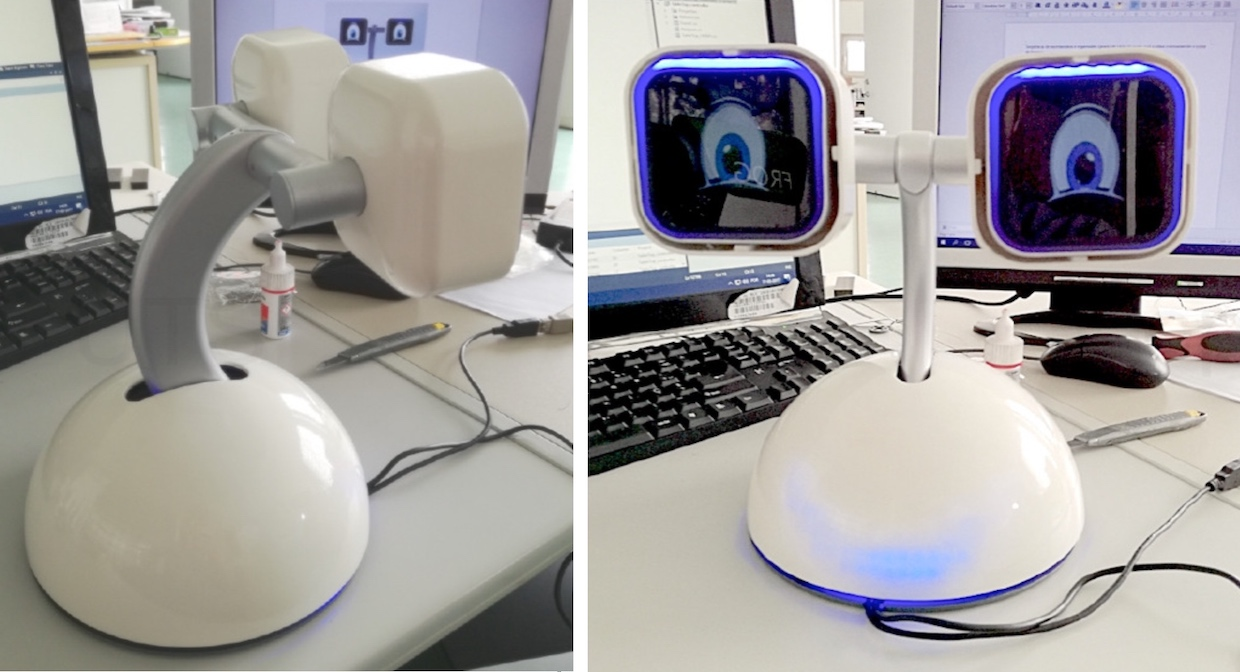
\includegraphics[width=\linewidth]{mirage/haru.jpeg}
%     \captionof{figure}{The HARU Robot.}
%     \label{fig:mirage:haru}
% } (See~\cref{fig:mirage:haru})
% The robot is fitted with cameras and a microphone array for visual and audio sensing.
% The array is circular with 6.5~cm radius, featuring 7 sensors.

% In ongoing work we are evaluating the \ac{MIRAGE} framework on real-world multichannel
% Not only that but you also use the better performing CNN_VN architecture from chapter 6. You need to mention this here.

% \newcommand{\MIRAGECNN}{\ensuremath{\mathtt{MIRAGE-CNN}_{\calV_\calN}}}
% \subsection{Multi-channel synthetic-data scenario}
% In this section, we compare the baseline \ac{SRP-PHAT} algorithm with the proposed approach, \ac{MIRAGE}, on multichannel synthetic data generated with the Python library \library{pyroomacoustics}\sidenote{\href{https://github.com/LCAV/pyroomacoustics}{\library{pyroomacoustics\ExternalLink}}}.
% In the \ac{SRP-PHAT} algorithm, we uses GCC-PHAT for TDOA estimation and its implementation is provided of the same toolbox we used for aggregating the local angular spectra (see Sidenotes~\ref{note:mbss} and ~\ref{note:mbss:para}).
% This time we use the more robust \ac{DNN} model based on \ac{CNN} trained with the Gaussian-based log-likelihood of~\cref{eq:lantern:gausslog}, dubbed here as $\MIRAGECNN$.
% We recall that the model is specifically trained and validated on white noise sources.
% \\The data are generated to match the design of the HARU's microphone array placed on top of a table:
% the 7 microphones are at most 15~cm from the close-surface, placed 13~cm from each other, with a little horizontal tilt ($\pm\ang{15}$);
% the other walls' absorption coefficients are uniformly sampled in $\kintervoo{0.5}{1}$ and the one of the close-surface is in $\kintervoo{0}{0.5}$.
% 200 different audio scenes have been generated including both white noise (wn) and speech source (sp) signals.
% Moreover, \ac{AWGN} noise was added to reach 10~dB \ac{SNR} level.
% The whole dataset design is similar to the one presented in~\cref{subsec:lantern:mlp}.

% \newthoughtpar{2D-SSL estimation on synthetic data}
% The performances are considered in terms of mean angular errors $\pm$ standard deviation in degree for both azimuth and elevation.
% 2D-\ac{DOA} estimation errors using the proposed approach and \ac{SRP-PHAT} are presented in~\cref{tab:mirage:ssl_syth}.
% For white noise source signals, \ac{SRP-PHAT} has better performances for both elevation and azimuth, but the proposed approach outperforms the baseline when the emitted signal is speech.
% It is interesting to notice that our DNN model trained and validated with white noise sources somewhat generalizes to speech sources.

% \begin{table}[t]
%     \begin{sidecaption}[]{
%         Mean squared errors and standard deviation in degrees for azimuth ($\theta$) and elevation ($\phi$). In bold the best records.
%     }[tab:mirage:ssl_syth]
%     \centering
%     \small
%     \begin{tabular*}{\linewidth}{@{\extracolsep{\fill}}lllllll@{}}
%         \toprule
%         & &  signal &  Error $\theta$  &  Error $\phi$ \\
%         \midrule
%         & \MIRAGECNN &   wn+n &  1.29 $\pm$   1.17 &   2.30 $\pm$   3.35 \\
%         & SRP-PHAT &   wn+n &  \textbf{0.49 $\pm$   0.6}1 &   \textbf{1.70 $\pm$   1.42} \\
%         \midrule
%         & \MIRAGECNN &  sp+n & \textbf{ 9.51 $\pm$ 15.84} &  \textbf{12.26  $\pm$  12.20} \\
%         & SRP-PHAT &  sp+n & 35.27 $\pm$  54.57 &  15.10 $\pm$  16.67 \\
%         \bottomrule
%     \end{tabular*}
%     \end{sidecaption}
% \end{table}

% \mynewline
% In~\cref{fig:mirage:synth_ssl_noise,fig:mirage:synth_ssl_speech}, the \ac{DOA} estimation results are reported as scatter-plots in a prediction-vs-ground-truth plane.
% When the test data consider broadband white noise souses, no difference is noticed in the performance between the two methods.
% However, when speech data are considered, \MIRAGECNN{} clearly outperforms the baseline in term of azimuth estimation.
% However, when looking at the elevation estimation, the performances of both of the method drop drastically .
% Unfortunately, this seems to contradict the good performances recorded for \ac{TDOE} estimation in~\cref{subsec:lantern:simple:cnn:results}, and further investigation is needed to explain this observation.

% \begin{figure}[t]
%     \begin{sidecaption}[]{
%         Scatter-plots (predictions-vs-ground-truth) for DOA estimation (azimuth and elevation) on synthetic data when the the source signal is \textbf{noise}.
%         The color map corresponds to different SNR level [dB] in the data.
%     }[fig:mirage:synth_ssl_noise]
%     \centering
%     \subfloat[azel_srp][2D-SSL with SRP-PHAT on noise data]{
%         \centering
%         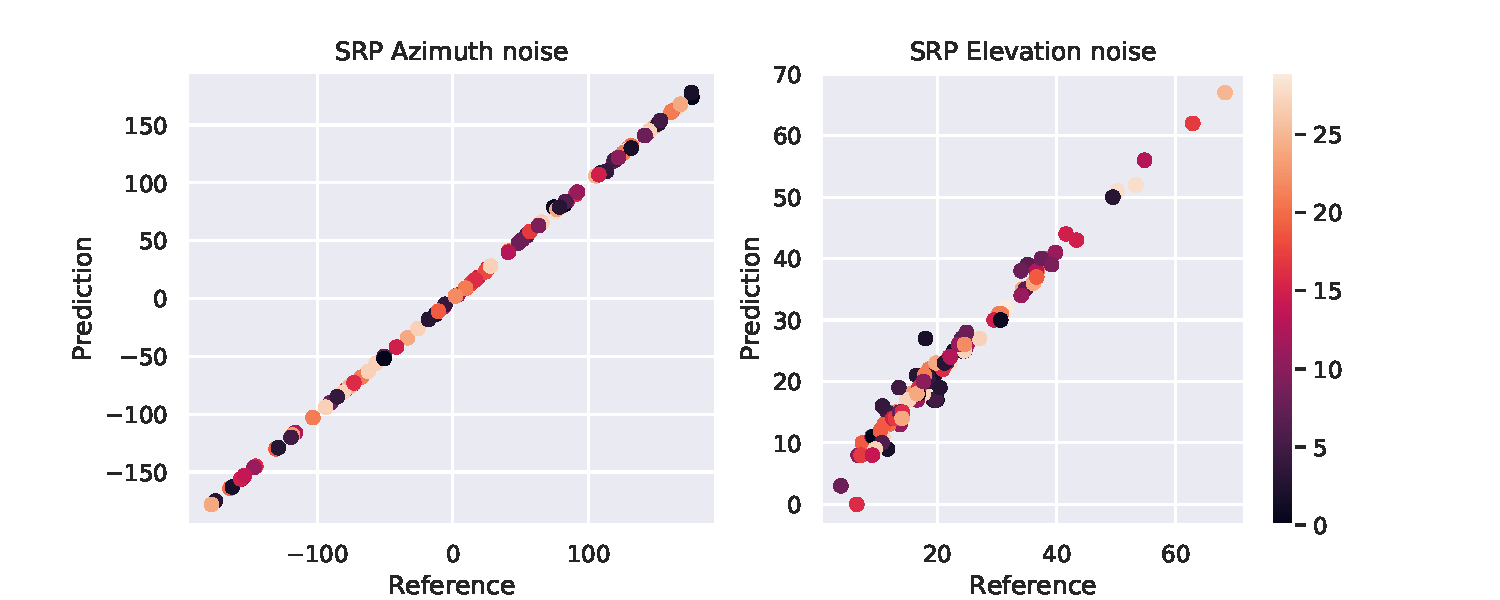
\includegraphics[width=\linewidth]{mirage/scatter_azel_estim_SRP_noise.pdf}
%         \label{fig:mirage:synth_ssl_noise_srp}
%     }
%     \hfill
%     \subfloat[azel_mirage][2D-SSL with  MIRAGE on noise data]{
%         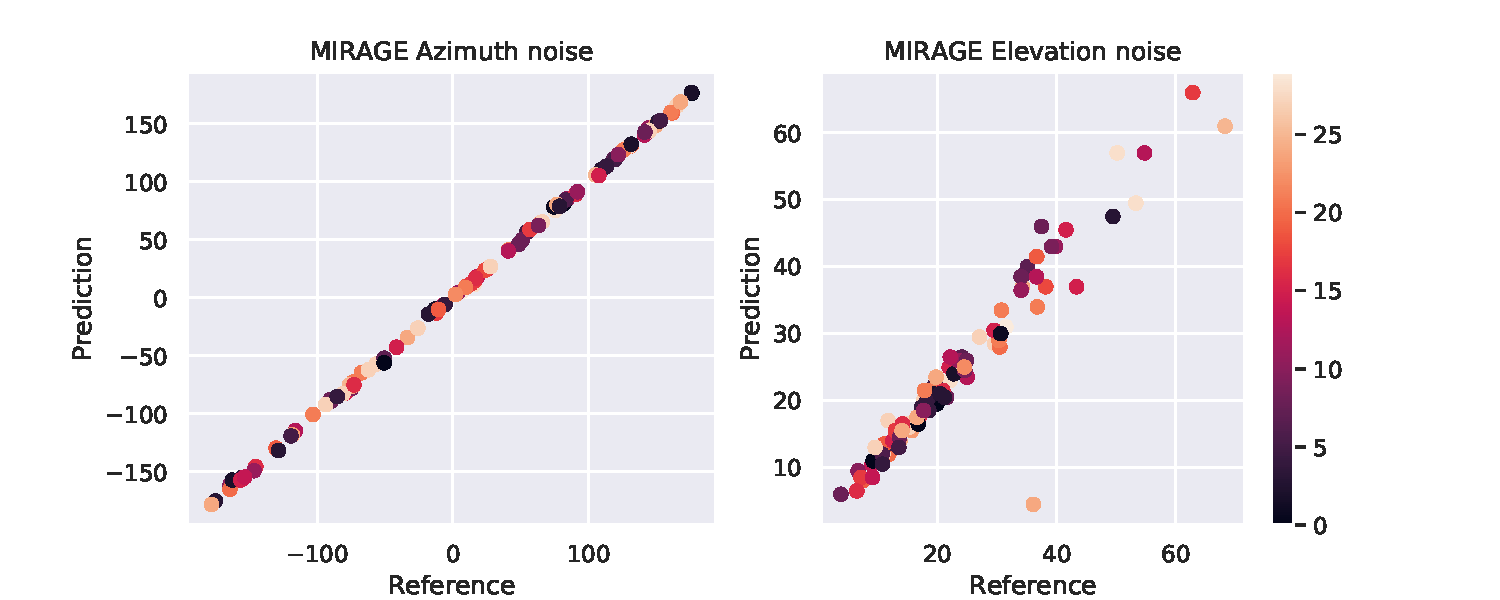
\includegraphics[width=\linewidth]{mirage/scatter_azel_estim_MIRAGE_noise.pdf}
%         \label{fig:mirage:synth_ssl_noise_mirage}
%     }
%     \end{sidecaption}
% \end{figure}

% \begin{figure}[t]
%     \begin{sidecaption}[]{
%         Scatterplots (predictions-vs-ground-truth) for DoA estimation (azimuth and elevation) on synthetic data when the the source signal is \textbf{speech}.
%         The color map corresponds to different SNR level [dB] in the data.
%     }[fig:mirage:synth_ssl_speech]
%     \centering
%     \subfloat[azel_srp][2D-SSL with SRP-PHAT on speech data]{
%         \centering
%         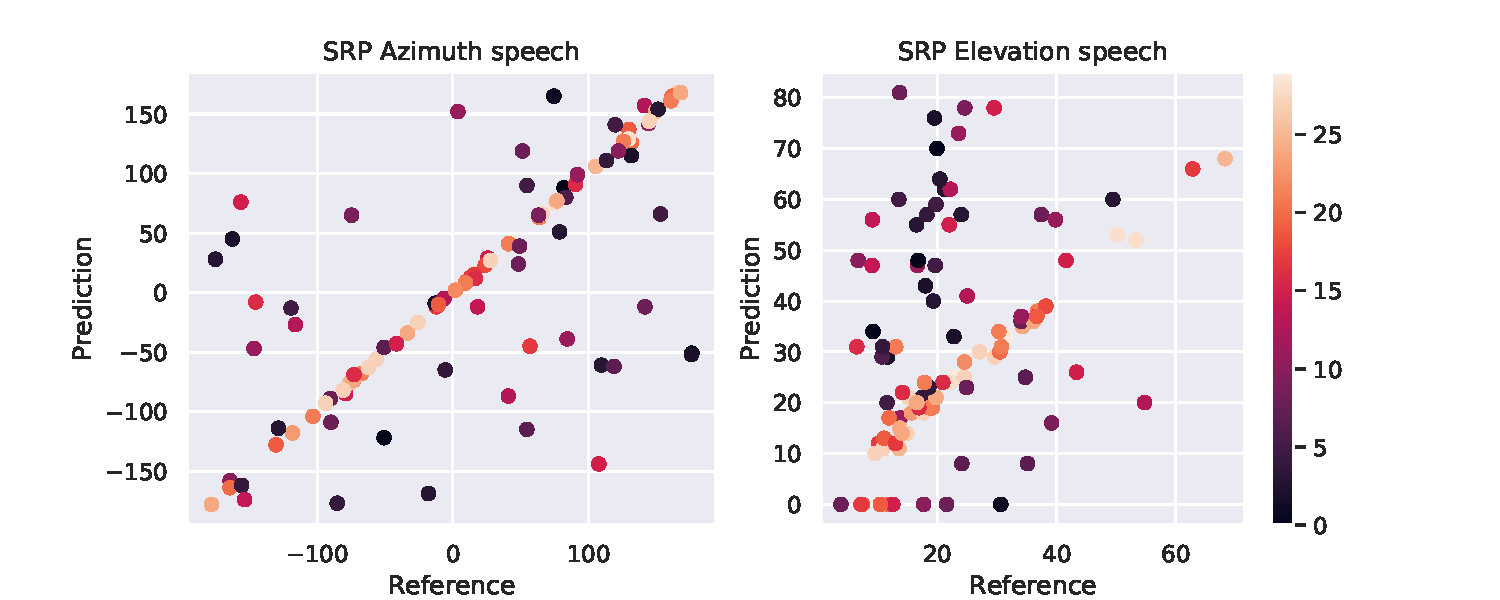
\includegraphics[width=\linewidth]{mirage/scatter_azel_estim_SRP_speech.pdf}
%         \label{fig:mirage:synth_ssl_speech_srp}
%     }
%     \hfill
%     \subfloat[azel_mirage][2D-SSL with  MIRAGE on speech data]{
%         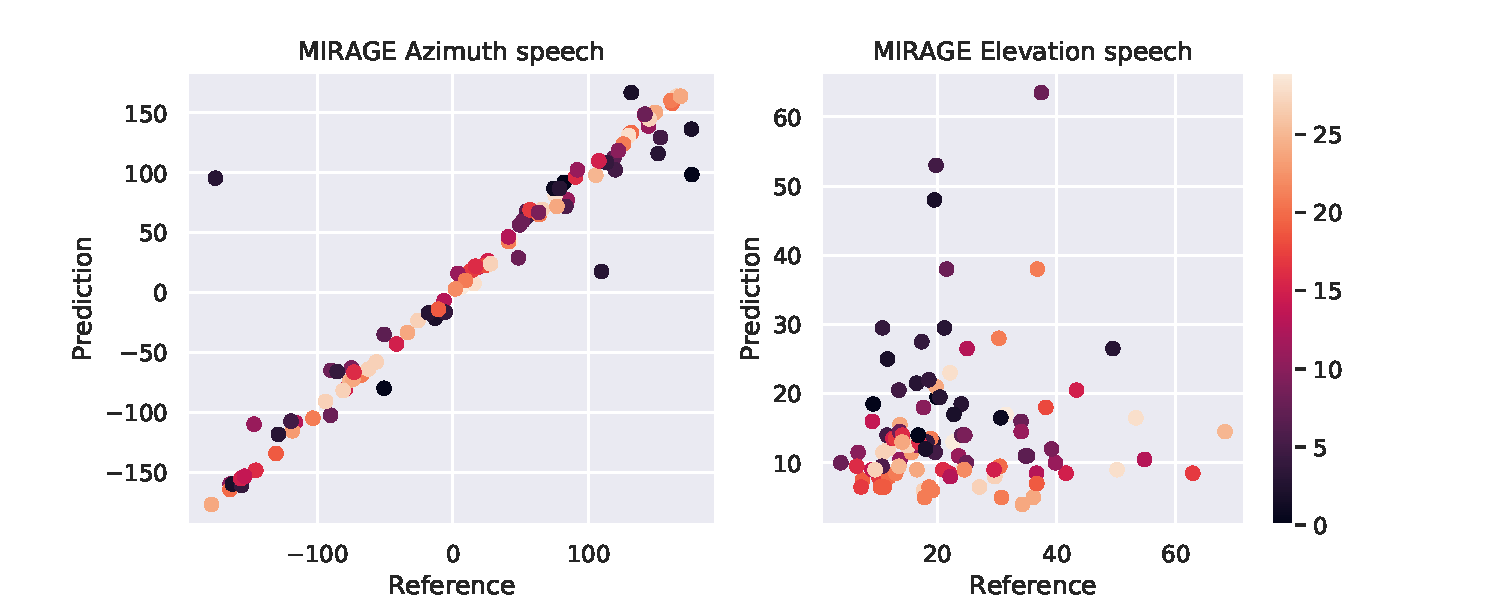
\includegraphics[width=\linewidth]{mirage/scatter_azel_estim_MIRAGE_speech.pdf}
%         \label{fig:mirage:synth_ssl_speech}
%     }
%     \end{sidecaption}
% \end{figure}

% \mynewline
% \newthought{Multi-channel real scenario} data were recorded with Haru's microphone array, as natural follow up of the work.
% The consider room setup is shown in~\cref{fig:mirage:room_exp}.
% However, due to lack of expertise and limitation in the measurement tools, these recording were discarded.
% Later, new data with the Haru robot were recorded, but the processing of their data is still work in progress.

% \begin{figure}[t]
%     \begin{fullwidth}
%     \centering
%     \subfloat[mu_spkr][HARU Array]{
%         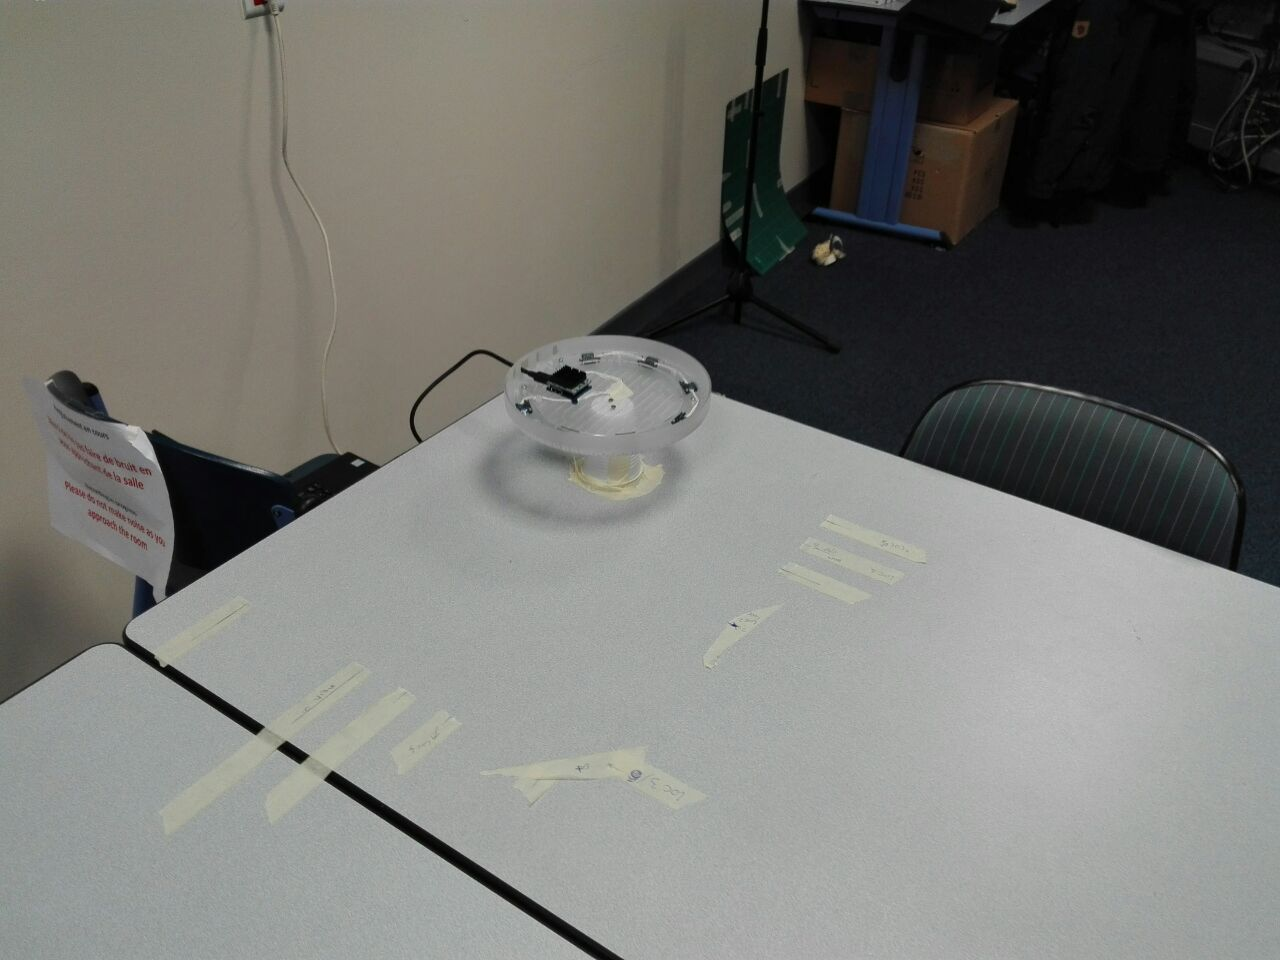
\includegraphics[width=0.32\textwidth]{figures/mirage/1_room_exp}}
%     \hfill
%     \subfloat[mu_spkr][Reflective table]{
%         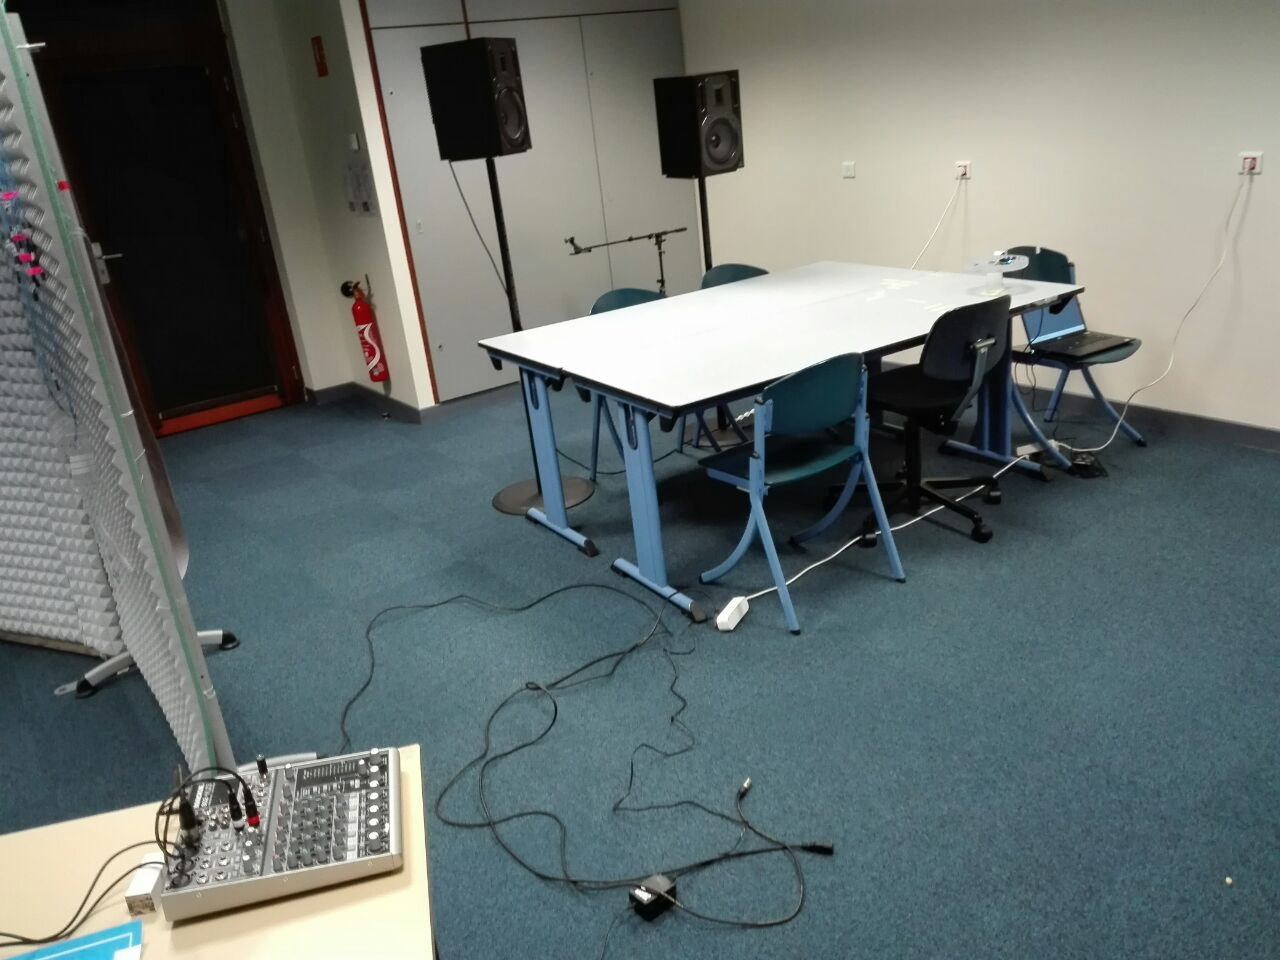
\includegraphics[width=0.32\textwidth]{figures/mirage/2_room_exp}}
%     \hfill
%     \subfloat[mu_univ][Detail]{
%             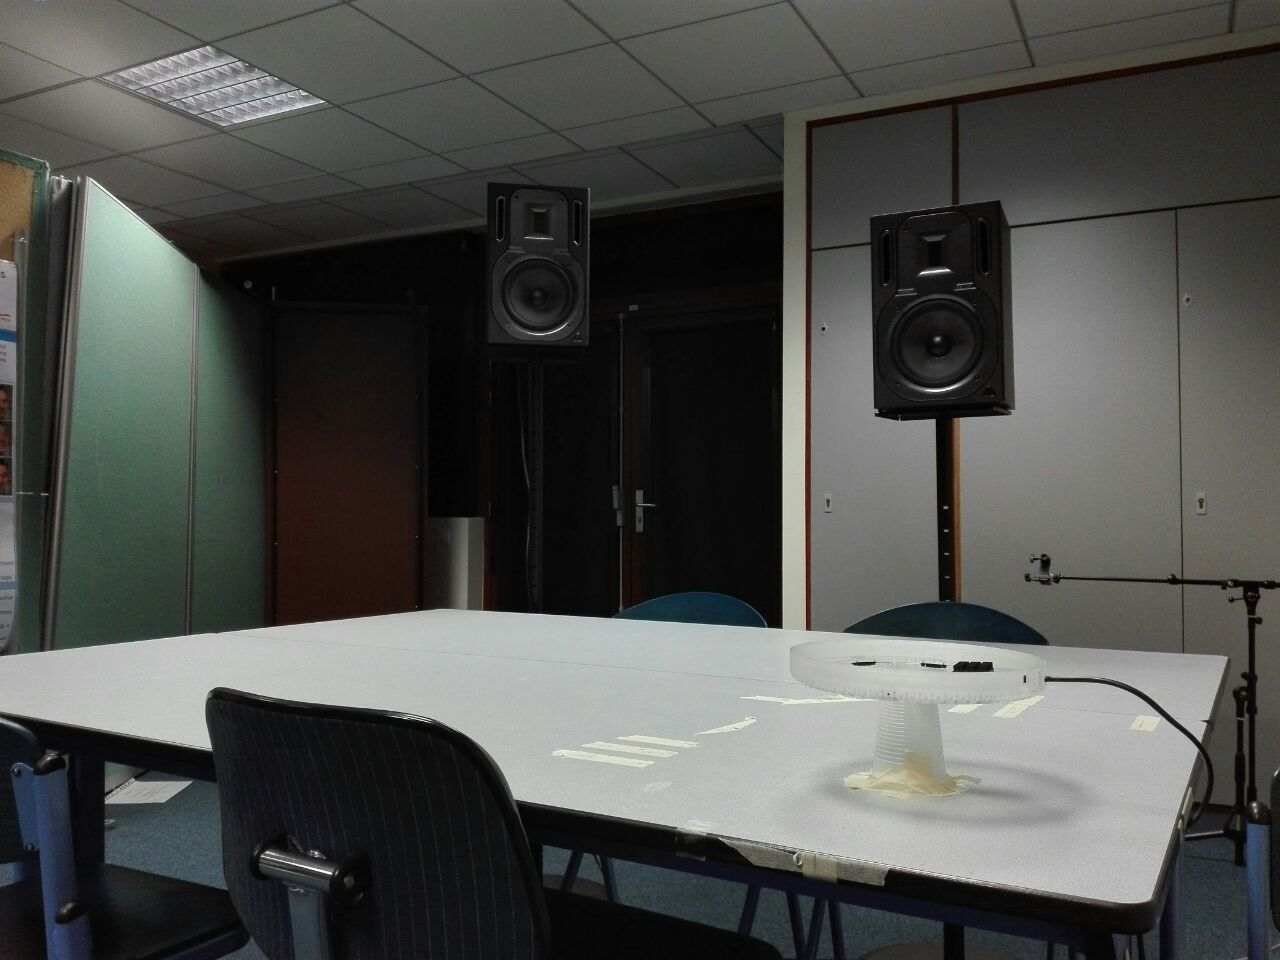
\includegraphics[width=0.32\textwidth]{figures/mirage/3_room_exp}}
%     \label{fig:mirage:room_exp}
%     \caption{Picture of the room and setup for recording real multichannel data with the HARU circular microphone array.}
%     \end{fullwidth}
% \end{figure}


% In this section, we compare the \ac{SRP-PHAT} algorithm (using GCC-PHAT for TDOA estimation) with the proposed approach, \MIRAGE/, on real multichannel recordings.
% This time we use the more robust \ac{DNN} model based on \ac{CNN} trained with the Gaussian-based log-likelihood of~\cref{eq:lantern:gausslog}, dubbed here as $\MIRAGECNN$.
% The real multichannel data were recorded with the HARU microphone circular array ($\numMics=7)$.
% The experiments were performed in a big office room 10~m $\times$ 15~m $\times$ 3~m with a reverberation time around 0.2 seconds.
% The HARU was placed on top of a table with a height of 0.10 m to simulate the close-reflector scenario, used to train the \ac{DNN} model.
% Two loudspeakers were used the emit one anechoic and normalized utterance from the TIMIT dataset and 10 seconds of white noise.
% The dataset consists of 5 different azimuthal positions and for each of them 2 different elevations yielding 10 different locations in space.
% The geometry of the setup was annotated using metric tape measures.


% \newthoughtpar{TDOA estimation and 2D-SSL performances on real data}
% As reported in~\cref{tab:mirage:tdoa_real}, the two methods are comparable both for speech and noise emitted signals even if \ac{SRP-PHAT} performs slightly better.
% In~\cref{fig:mirage:tdoa_real_pairs} the error on \ac{TDOA} estimation is shown of each microphone pair of the HARU.
% It can be seen that the error and the deviation are not homogeneous among the pairs.
% This might be due to some perturbations of the array's microphone positioning: the \ac{SRP-PHAT} method is only successful if the array's geometry is perfectly known \textit{a priori}.
% However, little misplacement leads to local distortion in the input angular spectra\sidenote{
%     In\citeonly{salvati2018exploiting}, the authors address this problem integrating \ac{SRP-PHAT} with a \ac{CNN} together.
% }.
% Moreover, the proposed approach needs the height of the robot (of each pair) as additional information, and again some perturbation can affect performances.

% \begin{table}[h]
%     \begin{sidecaption}[]{
%         Evaluation metrics (\ac{nRMSE}, \ac{RMSE}, \ac{STD}) for TDOA estimation and empirical computational times for different source signals.
%         Boldness denotes the best records.
%     }[tab:mirage:tdoa_real]
%     \centering
%     \small
%     \begin{tabular*}{\linewidth}{@{\extracolsep{\fill}}lllllll@{}}
%         \toprule
%         & &     signal &     nRMSE & RMSE &  STD &      time \\
%         \midrule
%         & \MIRAGECNN  &       noise &  0.26 &  0.94 &  0.57 &  0.26 \\
%         & SRP-PHAT &      noise &  0.20 &  0.62 &  0.57 &  6.48 \\
%         \midrule
%         & \MIRAGECNN &       speech &  0.40 &  1.38 &  0.99 &  0.24 \\
%         & SRP-PHAT &     speech &  0.32 &  0.82 &  1.08 &  4.02 \\
%         \bottomrule
%         \end{tabular*}
%     \end{sidecaption}
% \end{table}

% \begin{figure}
%     \begin{sidecaption}[]{
%         Violin-plots of the TDOA estimation errors (in samples) versus the microphone pairs in HARU for two different source signals on real data
%     }[fig:mirage:tdoa_real_pairs]
%         \centering
%         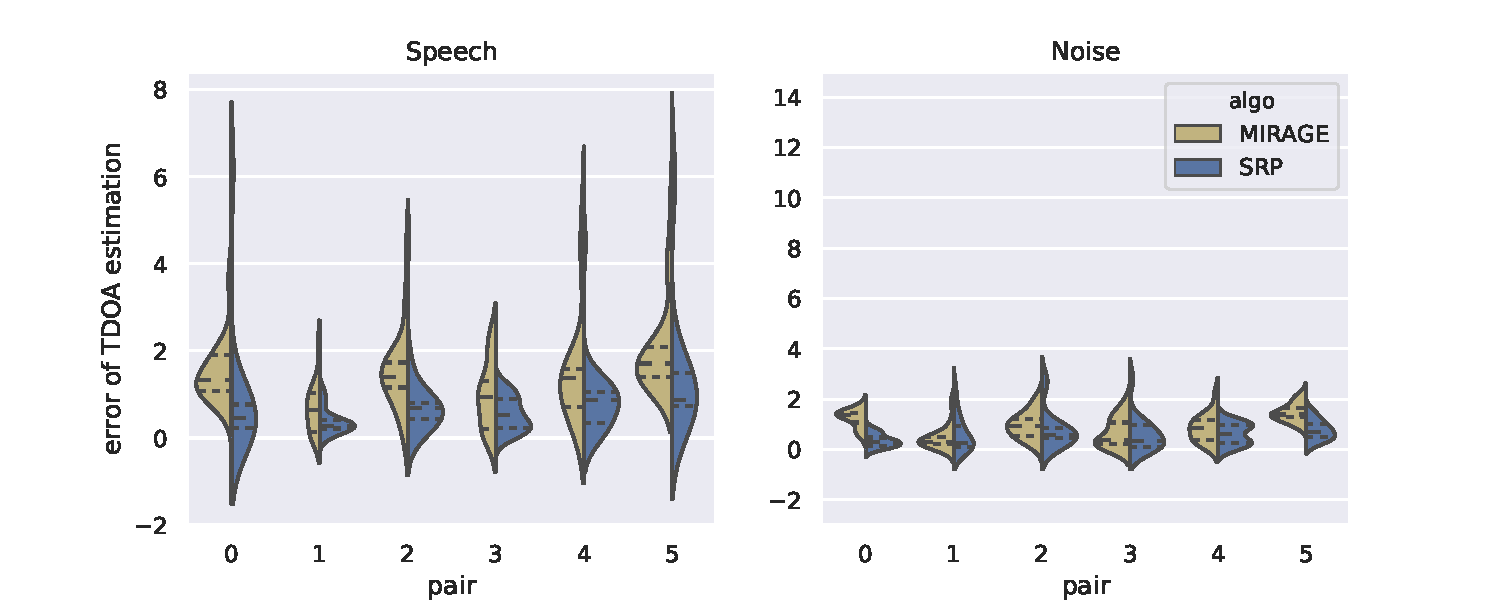
\includegraphics[trim={10 0 5 5},clip,width=\linewidth]{mirage/violinplot_tdoa_vs_pair_real.pdf}
%     \end{sidecaption}
% \end{figure}

% \mynewline
% Finally, we evaluate the performance of the methods for the 2D-\ac{SSL} task.
% The results in terms of \ac{RMSE} and standard deviation are shown in~\cref{tab:mirage:ssl_real}.
% When the signal emitted is speech, the CNN-based method outperforms the \ac{SRP-PHAT}.
% However, the latter seems to perform better for noise signals, even if comparable error margins are observed.

% \begin{table}[h]
%     \begin{sidecaption}[]{
%         Mean squared errors and standard deviations in degrees for estimation of azimuth ($\theta$) and elevation ($\phi$).
%         In bold the best records.
%     }[tab:mirage:ssl_real]
%     \centering
%     \small
%     \begin{tabular*}{\linewidth}{@{\extracolsep{\fill}}lllll@{}}
%         \toprule
%         &          &  signal &  Error $\theta$  &  Error $\phi$ \\
%         \midrule
%         & \MIRAGECNN   &   noise &   1.29 $\pm$   1.17 &     2.30 $\pm$  3.35 \\
%         & SRP-PHAT &   noise &   \textbf{0.49 $\pm$   0.61} &     \textbf{1.70 $\pm$  1.42} \\
%         \midrule
%         & \MIRAGECNN   &  speech & \textbf{  9.51 $\pm$  15.84} &    \textbf{12.26 $\pm$ 12.20} \\
%         & SRP-PHAT &  speech &  35.27 $\pm$  54.57 &    15.10 $\pm$ 16.67 \\
%         \bottomrule
%     \end{tabular*}

%     \end{sidecaption}
% \end{table}

% \mynewline
% \Cref{fig:mirage:real_ssl_noise,fig:mirage:real_ssl_speech} illustrate the distribution of the prediction of the methods with respect to the ground-truth in the azimuth-vs-elevation planes.
% We see that the predictions do not match the ground-truth properly.
% SRP-PHAT seems to overestimate elevation while predicting well the azimuth, especially for noise signals.
% MIRAGE seems to return more reasonable azimuth-elevation pairs.
% However, the elevation prediction seems to be almost constant across the points.
% Moreover, it seems that there is a constant offset or deviation, especially for azimuth prediction, suggesting that our real-data annotation was perhaps no accurate enough.

% \begin{figure}[h]
%     \begin{sidecaption}[]{
%         Scatterplots (azimuth-vs-elevation) for DOA estimation on real data when the the source signal is \textbf{noise}.
%         The colors indicate reference points (blue) and predicted ones (orange).
%     }[fig:mirage:real_ssl_noise]
%     \centering
%     \subfloat[azel_srp][2D-SSL with SRP-PHAT on real noise data]{
%         \centering
%         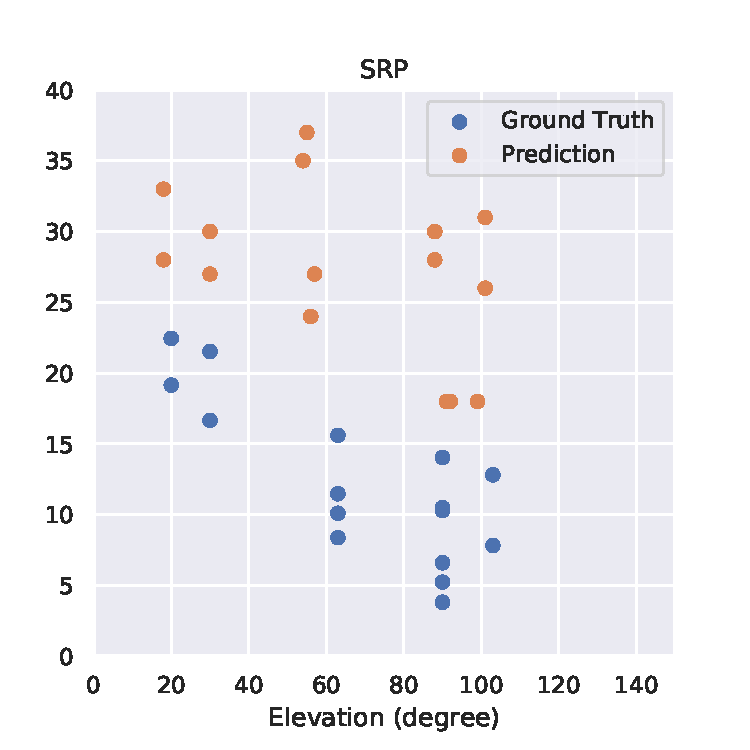
\includegraphics[width=0.47\linewidth]{mirage/scatterplot_SRP_broadband.pdf}
%         \label{fig:mirage:real_ssl_noise_srp}
%     }
%     \hfill
%     \subfloat[azel_mirage][2D-SSL with MIRAGE on real noise data]{
%         \centering
%         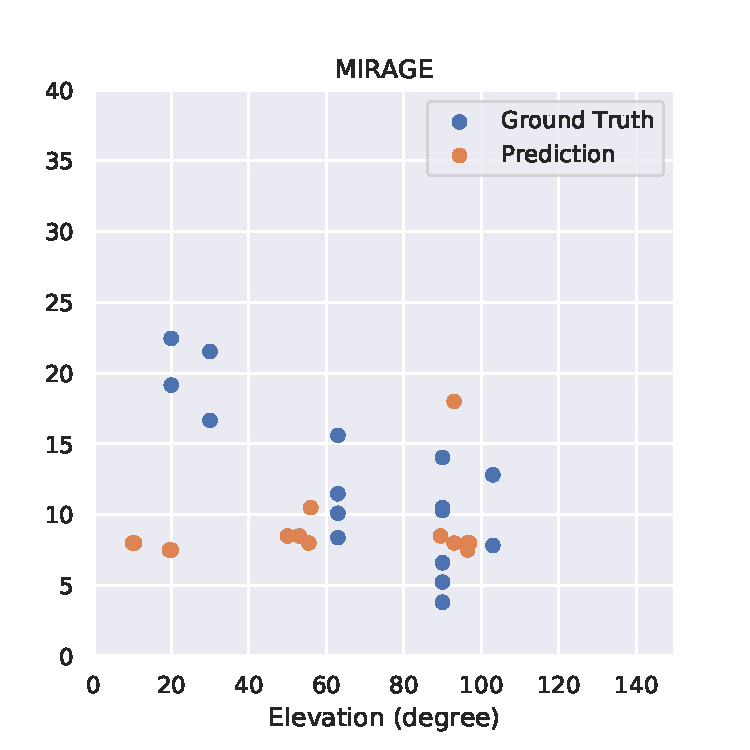
\includegraphics[width=0.47\linewidth]{mirage/scatterplot_MIRAGE_broadband.pdf}
%         \label{fig:mirage:real_ssl_noise_mirage}
%     }
%     \end{sidecaption}
% \end{figure}

% \begin{figure}[h]
%     \begin{sidecaption}[]{
%         Scatterplots (azimuth-vs-elevation) for DoA estimation on real data when the source signal is \textbf{speech}.
%         The colors indicate reference points (blue) and predicted ones (orange).
%     }[fig:mirage:real_ssl_speech]
%     \centering
%     \subfloat[azel_srp][2D-SSL with SRP-PHAT on real noise data]{
%         \centering
%         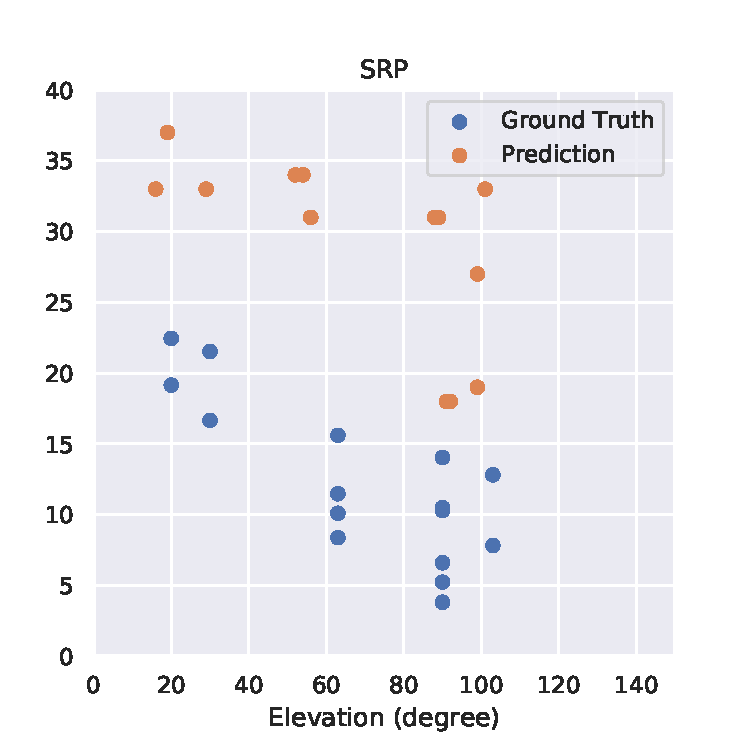
\includegraphics[width=0.47\linewidth]{mirage/scatterplot_SRP_speech.pdf}
%         \label{fig:mirage:real_ssl_speech_srp}
%     }
%     \hfill
%     \subfloat[azel_mirage][2D-SSL with MIRAGE on real noise data]{
%         \centering
%         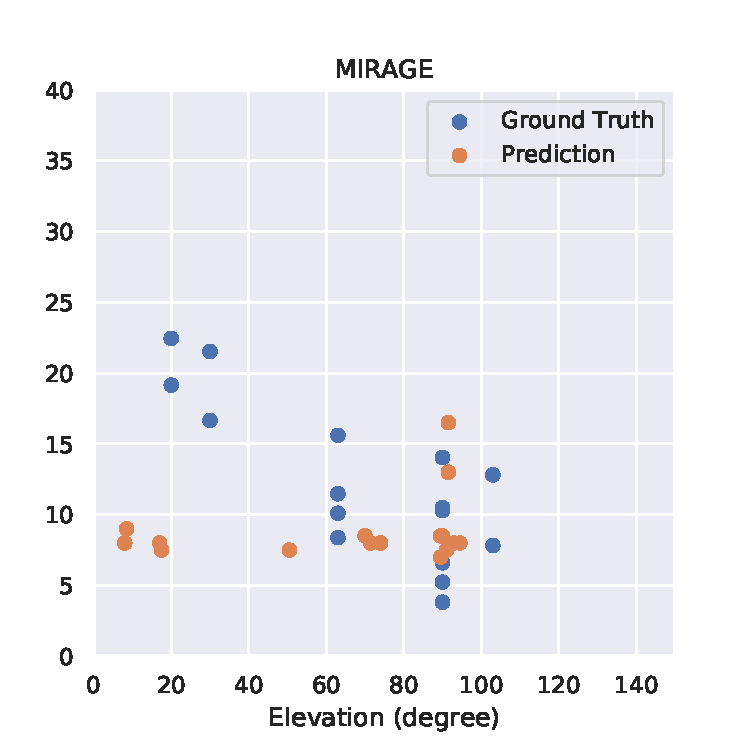
\includegraphics[width=0.47\linewidth]{mirage/scatterplot_MIRAGE_speech.pdf}
%         \label{fig:mirage:real_ssl_speech_mirage}
%     }
%     \end{sidecaption}
% \end{figure}


\section{Conclusion}
This chapter demonstrated how a simple echo model could boost an \ac{SSL} algorithm in strongly echoic conditions when microphones are placed close to a reflector.
We proposed to use a successful algorithm for multichannel \ac{SSL} on the virtual array created by image microphones.
In order to leverage such an array, the echoes' parameters need to be estimated.
To this end, we used the learning-based acoustic echo retrieval methods proposed in~\cref{ch:lantern}.
\\Preliminary results on synthetic data for stereophonic recordings prove the effectiveness of the proposed approach.
However, the task is still very challenging for both the proposed and baseline methods.
Considering the current knowledge, this is the first time an echo-aware method combines both knowledge-driven and data-driven approaches to \ac{SSL}.
The learning approach could still be significantly improved by considering other acoustic features (such as advance \ReTF/ methods), other architectures, and other challenges.
For instance, handling the missing frequencies of the speech while training on a broadband signal such as in~\citeonly{gaultier2017vast},
using physics-driven regularizers such as in~\citeonly{nabian2020physics} and make the learning phase independent of the array geometry.
Secondly, the approach need to be tested on real-world data, for which the $\dEchorate$ may be used as a valuable testing dataset.